\documentclass[11pt]{article}

\topmargin = 0mm
\textwidth = 150mm 
\oddsidemargin = 0mm

\usepackage[utf8]{inputenc}
\usepackage[russian]{babel}
\usepackage{graphicx}
\usepackage{caption}
\usepackage{amsmath}
\usepackage{listings}
\usepackage{float}
\usepackage{graphicx}
\usepackage{subfig}
\usepackage{bm}

\title{Методы оптимизации в машинном обучении \\
Отчет по практическому заданию №1}
\author{Коробов Павел, группа 617}

\begin{document}


\maketitle
\thispagestyle{empty}

\section{Введение.}
Данное практическое задание посвящено методам градиентного спуска и Ньютона, а также их сравнению. Рассматриваются различные стратегии выбора длины шага в градиентном спуске и методе Ньютона, зависимость поведения GD от числа обусловленности функции, сравнивается работа GD и метода Ньютона на оракуле логистической регрессии с реальными и модельными данными.
\section{Логистическая регрессия.}

\hspace{0.5cm} В задании нам понадобится оракул логистической регрессии. 

Пусть задана обучающая выборка $\{(a_1, b_1), \dots, (a_m, b_m)\}$, метки классов $b_i \in \{-1, 1\}$.
Требуется построить по ней линейный классификатор вида 
$$f(a) = sign(a^T x),$$ где $a$ -- признаковое описание объекта, а $x$ -- параметры модели.



Выпишем в матрично-векторной форме функцию потерь для логистической регрессии, а также ее градиент и гессиан:

$$L(x) = \frac1m 1_m^T 
				\ln(1 + \exp(-b \odot Ax)) 
				+ \frac{\lambda}2 \|{x}\|^2_2,$$

где $1_m^T = (1,\dots, 1)$ - вектор из единиц размерности $m$, $\odot$ обозначает поэлементное умножение векторов, функции применяются к векторам поэлементно.

$$\nabla L(x) = -\frac1m \left(\sigma(-b \odot Ax) \odot b \right)A + \lambda x$$

$$\nabla^2 L(x) = \frac1m A^{T} diag \left(\sigma(-b \odot Ax)\odot 
						        (1_m - \sigma(-b \odot Ax)) \right)A + \lambda I_n$$

\section{Эксперименты.}

\subsection{Траектория градиентного спуска на квадратичной функции}

Будем рассматривать квадратичные функции вида

\begin{equation}\label{eqn:quadratic}
f(x)=\frac12\langle A x, x\rangle-\langle b, x\rangle \tag{*}
\end{equation}

Рассмотрим две такие квадратичные функции, заданные матрицами \\
$A_1 = \begin{pmatrix}
1 & 0 \\
0 & 1.2 \\
\end{pmatrix}$ и
$A_2 = \begin{pmatrix}
1 & 0 \\
0 & 10 \\
\end{pmatrix}$ соответственно, и имеющие нулевые линейные части. Начальная точка для алгоритма градиентного спуска $x_0=(4, 1)$.

На рисунке \ref{fig:WellConditioned1} видно, что с хорошо обусловленной матрицей $A_1$ все методы хорошо справляются и нет отличий между стратегией с постоянной длиной шага $\alpha_k = 1$ и линейным поиском, использующим условия Армихо и Вульфа.


В случае, если за матрицу квадратичной части взять $A_2$ (рисунок \ref{fig:BadlyConditioned1}) мы видим, что стратегия с постоянной длиной шага, равной 1.0, приводит к бесконечному удалению от оптимальной точки, но алгоритм сойдется, если подобрать меньшую длину шага. Использование сильных условий Вульфа помогло алгоритму сойтись немного быстрее, чем при использовании условия Армихо (за 16 итераций вместо 23).

При изменении начальной точки на $x_0=(1, 4)$ ситуация с функцией, заданной матрицей $A_1$, не меняется (рисунок \ref{fig:WellConditioned2}),
а в случае функции, заданной матрицей $A_2$ можно увидеть, что использование условий Вульфа заметно помогает в сравнении с выбором длины шага по условиям Армихо (рисунок \ref{fig:BadlyConditioned2}).

Можно сделать вывод, что стратегия выбора, использующая сильные условия Вульфа, наиболее устойчива к плохой обусловленности квадратичной функции.

\begin{figure}[h!p]
	\centering
	\begin{tabular}[c]{cc}
		\subfloat[Константная стратегия с длиной шага 1.0]{
    		\includegraphics[width=.5\textwidth]{{pics/traj_low_cond_(x_0=(4,1))/Constant_1.0}.png}
 		} &

		\subfloat[Константная стратегия с длиной шага 0.1]{
    		\includegraphics[width=.5\textwidth]{{pics/traj_low_cond_(x_0=(4,1))/Constant_0.1}.png}
 		} \\

		\subfloat[Армихо]{
    		\includegraphics[width=.5\textwidth]{{pics/traj_low_cond_(x_0=(4,1))/Armijo}.png}
	 	} &

		\subfloat[Вульф]{
    		\includegraphics[width=.5\textwidth]{{pics/traj_low_cond_(x_0=(4,1))/Wolfe}.png}
	 	}
   \end{tabular}
   \captionsetup{justification=centering,margin=2cm}
   \caption{Траектории при оптимизации методом градиентного спуска квадратичной функции, заданной матрицей $A_1$, $x_0=(4, 1)$}
\label{fig:WellConditioned1}
\end{figure} 

\begin{figure}[h!p]
	\centering
	\begin{tabular}[c]{cc}
		\subfloat[Константная стратегия с длиной шага 1.0]{
    		\includegraphics[width=.5\textwidth]{{pics/traj_high_cond_(x_0=(4,1))/Constant_1.0}.png}
    		\label{fig:StrategyA}%
 		} &

		\subfloat[Константная стратегия с длиной шага 0.1]{
    		\includegraphics[width=.5\textwidth]{{pics/traj_high_cond_(x_0=(4,1))/Constant_0.1}.png}
    		\label{fig:StrategyB}%
 		} \\

		\subfloat[Армихо]{
    		\includegraphics[width=.5\textwidth]{{pics/traj_high_cond_(x_0=(4,1))/Armijo}.png}
    		\label{fig:StrategyC}%
	 	} &

		\subfloat[Вульф]{
    		\includegraphics[width=.5\textwidth]{{pics/traj_high_cond_(x_0=(4,1))/Wolfe}.png}
    		\label{fig:StrategyD}%
	 	}
   \end{tabular}
   \captionsetup{justification=centering,margin=2cm}
   \caption{Траектории при оптимизации методом градиентного спуска квадратичной функции, заданной матрицей $A_2$, $x_0=(4, 1)$}
\label{fig:BadlyConditioned1}
\end{figure} 

\begin{figure}[h!p]
	\centering
	\begin{tabular}[c]{cc}
		\subfloat[Константная стратегия с длиной шага 1.0]{
    		\includegraphics[width=.5\textwidth]{{pics/traj_low_cond_(x_0=(1,4))/Constant_1.0}.png}
    		\label{fig:StrategyA}%
 		} &

		\subfloat[Константная стратегия с длиной шага 0.1]{
    		\includegraphics[width=.5\textwidth]{{pics/traj_low_cond_(x_0=(1,4))/Constant_0.1}.png}
    		\label{fig:StrategyB}%
 		} \\

		\subfloat[Армихо]{
    		\includegraphics[width=.5\textwidth]{{pics/traj_low_cond_(x_0=(1,4))/Armijo}.png}
    		\label{fig:StrategyC}%
	 	} &

		\subfloat[Вульф]{
    		\includegraphics[width=.5\textwidth]{{pics/traj_low_cond_(x_0=(1,4))/Wolfe}.png}
    		\label{fig:StrategyD}%
	 	}
   \end{tabular}
   \captionsetup{justification=centering,margin=2cm}
   \caption{Траектории при оптимизации методом градиентного спуска квадратичной функции, заданной матрицей $A_1$, $x_0=(1, 4)$}
\label{fig:WellConditioned2}
\end{figure} 

\begin{figure}[h!p]
	\centering
	\begin{tabular}[c]{cc}
		\subfloat[Константная стратегия с длиной шага 1.0]{
    		\includegraphics[width=.5\textwidth]{{pics/traj_high_cond_(x_0=(1,4))/Constant_1.0}.png}
    		\label{fig:StrategyA}%
 		} &

		\subfloat[Константная стратегия с длиной шага 0.1]{
    		\includegraphics[width=.5\textwidth]{{pics/traj_high_cond_(x_0=(1,4))/Constant_0.1}.png}
    		\label{fig:StrategyB}%
 		} \\

		\subfloat[Армихо]{
    		\includegraphics[width=.5\textwidth]{{pics/traj_high_cond_(x_0=(1,4))/Armijo}.png}
    		\label{fig:StrategyC}%
	 	} &

		\subfloat[Вульф]{
    		\includegraphics[width=.5\textwidth]{{pics/traj_high_cond_(x_0=(1,4))/Wolfe}.png}
    		\label{fig:StrategyD}%
	 	}
   \end{tabular}
   \captionsetup{justification=centering,margin=2cm}
   \caption{Траектории при оптимизации методом градиентного спуска квадратичной функции, заданной матрицей $A_2$, $x_0=(1, 4)$}
\label{fig:BadlyConditioned2}
\end{figure} 

\newpage
\subsection{Зависимость числа итераций градиентного спуска от числа обусловленности и размерности пространства}

Будем изучать зависимость числа итераций градиентного спуска от числа обусловленности на квадратичной функции вида \eqref{eqn:quadratic} с диагональной матрицей $A$, где первый элемент на диагонали равен $1$, последний -- $\kappa$, а остальные взяты из равномерного распределения на отрезке $[1, \kappa]$, компоненты вектора линейной части берутся из равномерного распределения на отрезке $[-1, 1]$.

Построим усредненные по ста запускам кривые для числа переменных $n = 2, 10, \\100, 1000$,
$\kappa$ будем менять в диапазоне от 1 до 1000. Будем также показывать прозрачным цветом коридор стандартного отклонения.


\begin{figure}[h!p]
	\centering
    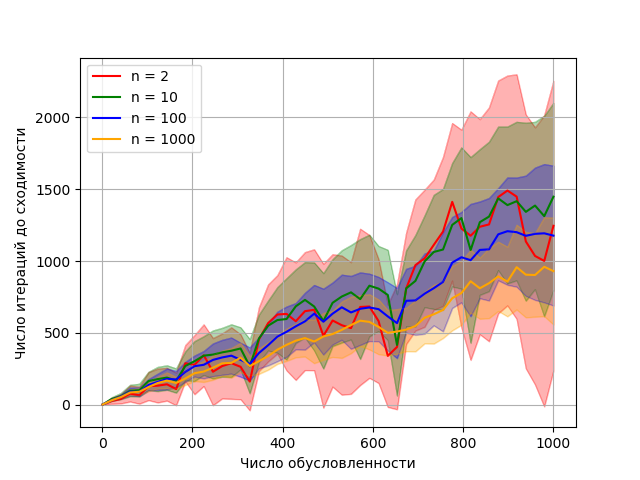
\includegraphics[width=1.0\textwidth]{pics/iterations_vs_condition_number.png}
\captionsetup{justification=centering}
\caption{Зависимость числа итераций GD от числа обусловленности при разных $n$ на нескольких запусках}
\end{figure}

По всем кривым можно заключить, что число итераций возрастает с числом обусловленности.

Можно увидеть, что кривые, соответствующие $n=1000$, $n=100$, и $n=10$ явно упорядочены на графике снизу вверх. Значения, соответствующие $n = 2$ при этом имеют самое большое стандартное отклонение, и самое большое число итераций мы можем получить именно при $n=2$.

Можно заключить, что с ростом размерности число итераций менее чувствительно к плохой обусловленности функции, или, иначе говоря, число итераций обратно зависит от размерности задачи.

\subsection{Оптимизация вычислений в градиентном спуске}

Сравним наивную и оптимизированную реализации оракула логистической регрессии на модельной выборке.
Возьмём $n = 10000, m = 8000$. Компоненты матрицы объектов-признаков $A$ сегенерируем из $\mathcal{N}(0, 1)$. Метки классов -- $sign(\mathcal{N}(0, 1))$.


\begin{figure}[h!p]
	\centering
    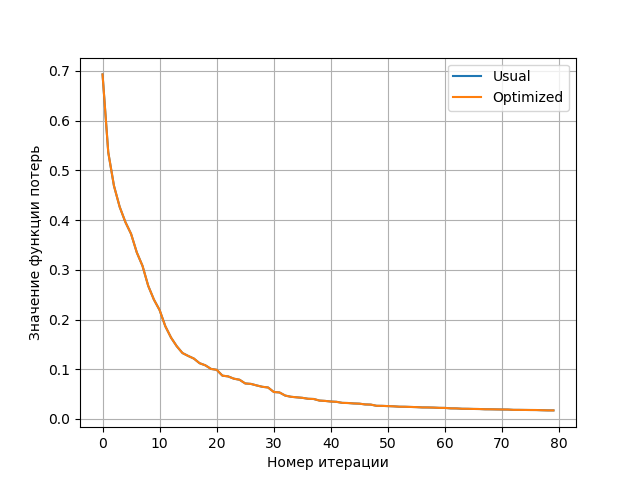
\includegraphics[width=.7\textwidth]{pics/logreg_values.png}
   \captionsetup{justification=centering,margin=2cm}
   \caption{Графики значений функции потерь логистической регрессии при оптимизации градиентным спуском}
\end{figure}

Графики значений функций, конечно же, одинаковы, потому что одинаковы начальные приближения, а вычисления никак не изменились, а лишь были исключены избыточные матрично-векторные умножения.

\begin{figure}[h!p]
	\centering
    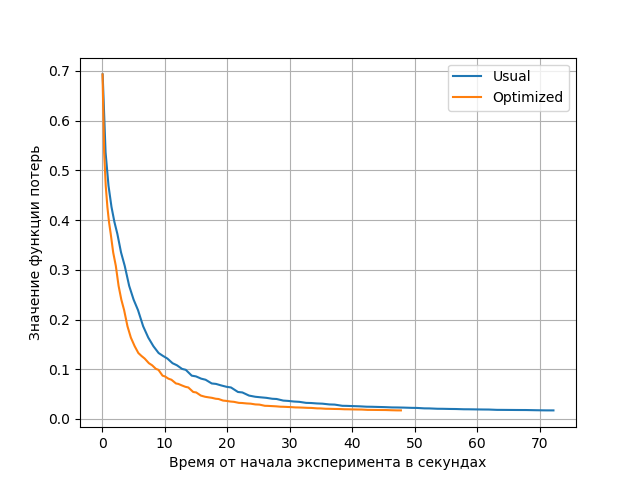
\includegraphics[width=0.7\textwidth]{pics/logreg_loss_value_vs_time.png}
\captionsetup{justification=centering}
\caption{График значений функции потерь логистической регрессии в зависимости от времени}
\label{fig:optimized_values_vs_time}
\end{figure}

\begin{figure}[h!p]
	\centering
    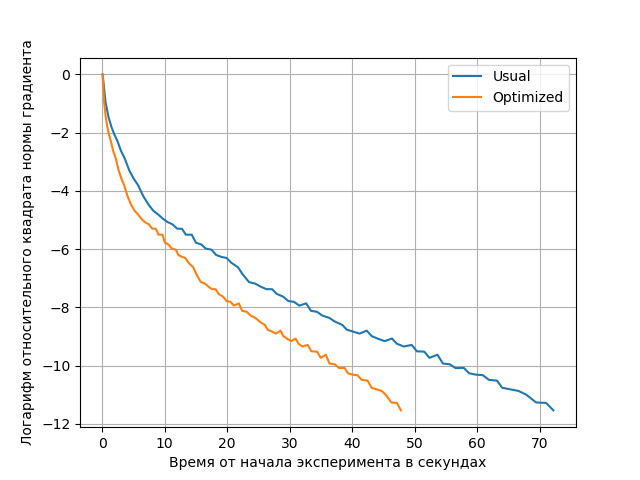
\includegraphics[width=0.7\textwidth]{pics/logreg_grad_norm_vs_time.png}
\captionsetup{justification=centering}
\caption{График зависимости $
\log\left(\left\|\nabla L\left(x_{k}\right)\right\|_{2}^{2} /\left\|\nabla L\left(x_{0}\right)\right\|_{2}^{2}\right)
$ от времени}
\label{fig:optimized_grad_vs_time}
\end{figure}

По рисункам \ref{fig:optimized_values_vs_time} и \ref{fig:optimized_grad_vs_time}  видно, что с оптимизированным оракулом GD сходится быстрее по времени.

\newpage
\subsection{Сравнение методов градиентного спуска и Ньютона на
реальной задаче логистической регрессии}

Сравним методы градиентного спуска и Ньютона на реальных наборах данных с сайта LIBSVM: $w8a$, $gisette$ и
$real$-$sim$.

Взглянем на число объектов $m$ и число признаков $n$ в выборках:
\begin{center}
\begin{tabular}{|c|c|c|} 
 \hline
 Данные & $m$ & $n$ \\ [0.5ex] 
 \hline\hline
 w8a & 49749 & 300 \\ 
 \hline
 gisette & 6000 & 5000 \\ 
 \hline
 real-sim & 72309 & 20958 \\ 
 \hline
\end{tabular}
\end{center}

Будем иметь в виду, что на итерации градиентного спуска и метода Ньютона мы тратим $O(mn)$ (самые дорогие операции - матрично-векторные произведения при подсчете градиента) и $O(n^2(m + n))$ (матричное произведение при расчете гессиана + разложение Холецкого для решения СЛАУ)
соответственно. Сложность метода Ньютона на последнем наборе данных слишком высока, поэтому на нём мы будем рассматривать только градиентный спуск.

На наборе данных $w8a$ итерации метода Ньютона не слишком дороги и точность его итераций позволяет ему сойтись за меньшее время, но этот пример вряд ли показывает практическое преимущество методоа Ньютона из-за того, что оба метода сошлись примерно за одну секунду.

На наборе данных $gisette$ метод Ньютона делает всего несколько итераций до сходимости, но существенно более дорогих, чем итерации градиентного спуска.

На наборе данных $real$-$sim$ градиентный спуск сошелся за 50 секунд, а метод Ньютона со сложностью, получаемой на этом наборе данных, запускать просто нецелесообразно.


\begin{figure}[h!p]
	\centering
	\begin{tabular}[c]{cc}
		\subfloat[Значения функции потерь против времени]{
    		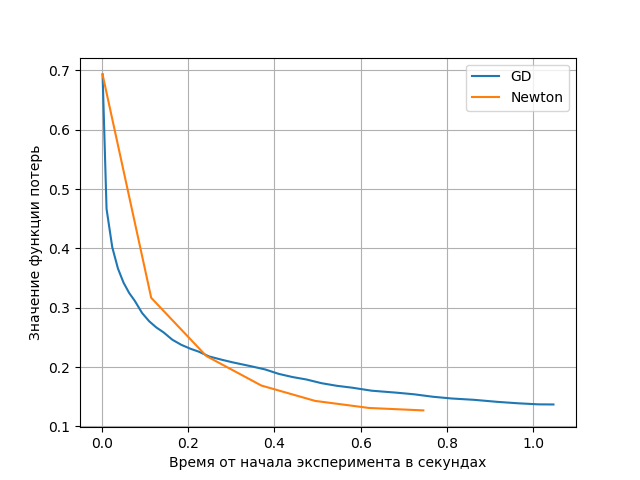
\includegraphics[width=.5\textwidth]{pics/logreg_loss_value_vs_time_w8a.png}
 		} &

		\subfloat[$
					\log\left(\left\|\nabla L\left(x_{k}\right)\right\|_{2}^{2} /\left						\|\nabla L\left(x_{0}\right)\right\|_{2}^{2}\right)
				  $ против времени]{
    		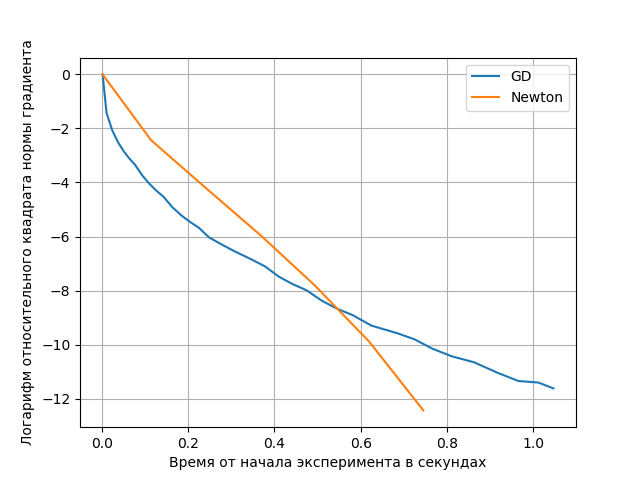
\includegraphics[width=.5\textwidth]{pics/logreg_grad_norm_vs_time_w8a.png}
 		}
   \end{tabular}
   \captionsetup{justification=centering}
   \caption{Сравнение градиентного спуска и метода Ньютона на $w8a$}
\label{fig:w8a}
\end{figure} 

\begin{figure}[h!p]
	\centering
	\begin{tabular}[c]{cc}
		\subfloat[Значения функции потерь против времени]{
    		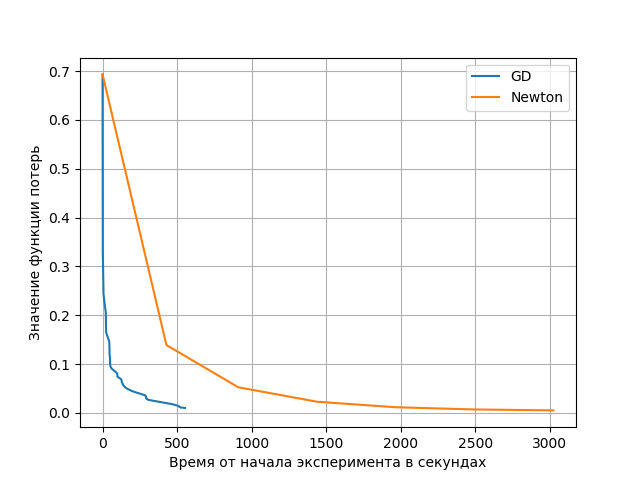
\includegraphics[width=.5\textwidth]{pics/logreg_loss_value_vs_time_gisette_scale.png}
 		} &

		\subfloat[$
					\log\left(\left\|\nabla L\left(x_{k}\right)\right\|_{2}^{2} /\left						\|\nabla L\left(x_{0}\right)\right\|_{2}^{2}\right)
				  $ против времени]{
    		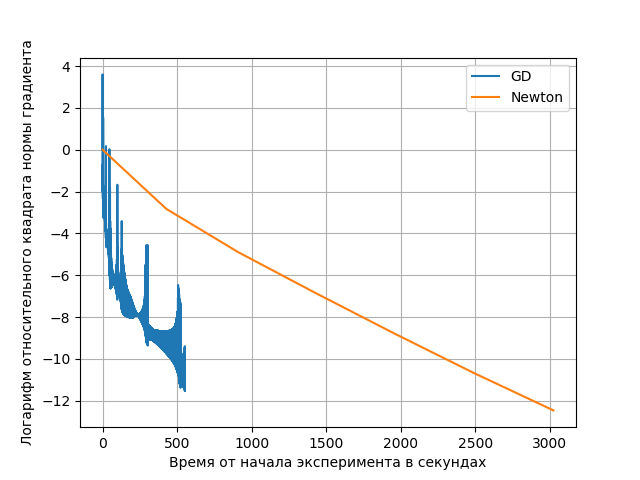
\includegraphics[width=.5\textwidth]{pics/logreg_grad_norm_vs_time_gisette_scale.png}
 		}
   \end{tabular}
   \captionsetup{justification=centering}
   \caption{Сравнение градиентного спуска и метода Ньютона на $gisette$}
\label{fig:gisette}
\end{figure} 

\newpage

\begin{figure}[h!p]
	\centering
	\begin{tabular}[c]{cc}
		\subfloat[Значения функции потерь против времени]{
    		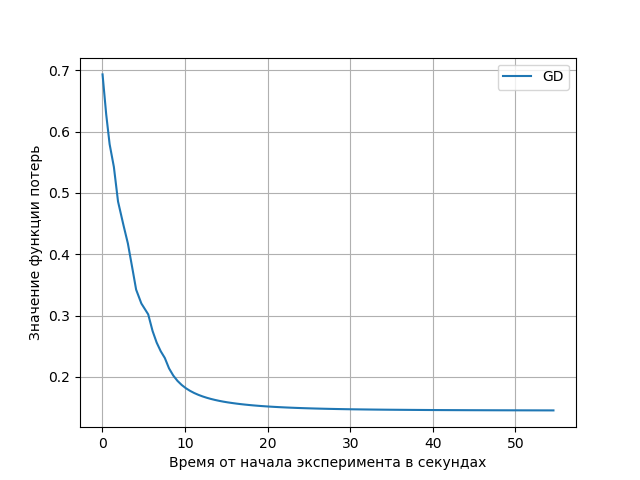
\includegraphics[width=.5\textwidth]{pics/logreg_loss_value_vs_time_real-sim.png}
 		} &

		\subfloat[$
					\log\left(\left\|\nabla L\left(x_{k}\right)\right\|_{2}^{2} /\left						\|\nabla L\left(x_{0}\right)\right\|_{2}^{2}\right)
				  $ против времени]{
    		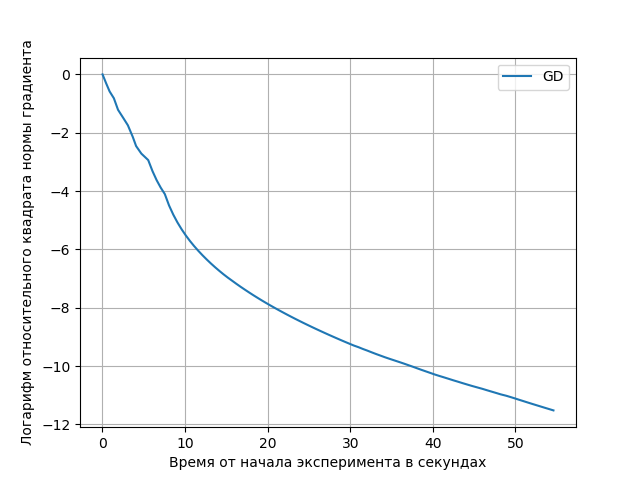
\includegraphics[width=.5\textwidth]{pics/logreg_grad_norm_vs_time_real-sim.png}
 		}
   \end{tabular}
   \captionsetup{justification=centering}
   \caption{Градиентный спуск на $real$-$sim$}
\end{figure} 

\subsection{Стратегия выбора длины шага в градиентном спуске}

Исследуем, какие стратегии являются лучшими на примерах логистической регрессии и оптимизации квадратичной функции.
Сравним стратегию с постоянной длиной шага, стратегию, использующую условие Армихо, и стратегию, использующую сильные условия Вульфа. Будем сравнивать их, перебирая длину шага $c$, параметры $c_1$ и $c_2$ соответственно. 

Задача логистической регрессии генерируется так же, как в эксперименте <<Оптимизация вычислений в градиентном спуске>>, при этом $n = 1000$, $m = 2000$.

Квадратичная функция генерируется следующим образом: положим $n=500$, генерируется диагональная матрица $\tilde{A}$ со значениями из $U([1, 20])$, затем генерируется ортогональная матрица $C$. $A = C^T \tilde{A} C$, компоненты $b$ генерируются из $\mathcal{N}(0, 1)$. 

Будем сравнивать стратегии на трёх начальных точках: $0_n$, случайной точке и либо $1_n$ для логистической регрессии, либо на точке, полученной из минимума прибавлением нормального шума, для квадратичной функции.

К кривым на графиках добавлен небольшой случайный шум для лучшей читаемости графиков, так как при некоторых значениях параметров некоторые кривые совпадают. 

На рисунке \ref{fig:gd_strategies_logreg} видим, что стратегии с условиями Вульфа со значениями \\ $c_2 < 1$ позволяют совершить GD меньше итераций, чем остальные. 
Стратегия с $c_2=1.5$ находится в одном кластере со стратегией Армихо, что понятно: мы не требуем уменьшения производной по направлению и существенным остаётся только условие Армихо.
Лучшая -- стратегия Вульфа с $c_2=0.9$. Все представленные стратегии Армихо ведут себя одинаково, в одном кластере с ними, как было сказано выше -- Вульф с $c_2=1.5$ и постоянный шаг $c=1$. Меньшие значения постоянного шага, как и ожидается, приводят к большему числу итераций алгоритма.

На рисунке \ref{fig:gd_strategies_quadratic}, однако, для двух из трёх начальных точек  лучшей является стратегия с условиями Вульфа с $c_2 = 1.5$, для третьей точки лучшими оказываются стратегии, использующие условие Армихо. С другой стороны, для третьей точки все стратегии сошлись примерно в районе 17-й итерации и разница заметна не так сильно, как на первых двух точках. Для первых двух точек также видно, что до какого-то момента лидирует стратегия с условием Армихо и $c_1=0.1$.

Вывод: линейный поиск помогает методам сойтись быстрее, чем константные стратегии, для логистической регрессии хороший выбор -- стратегия Вульфа с $c_2=0.9$, для квадратичной функции мы можем получить разные результаты в зависимости от начального приближения.

\begin{figure}[h!p]
	\centering
	\begin{tabular}[c]{cc}
		\subfloat[$x_0=0_n$]{
    		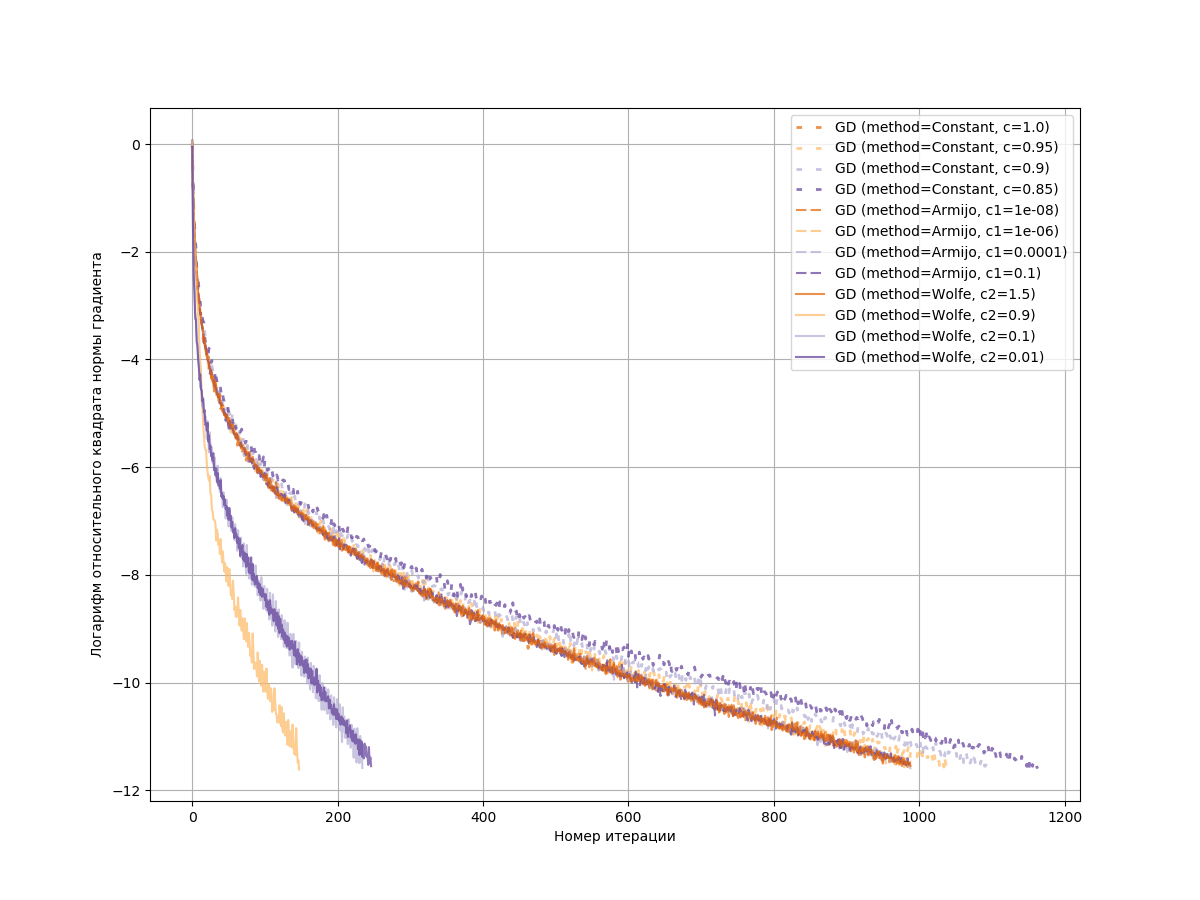
\includegraphics[width=.5\textwidth]{pics/logreg_GD_linear_search_strategies/x_0_0.png}
 		} &

		\subfloat[$x_0$ -- случайная точка]{
    		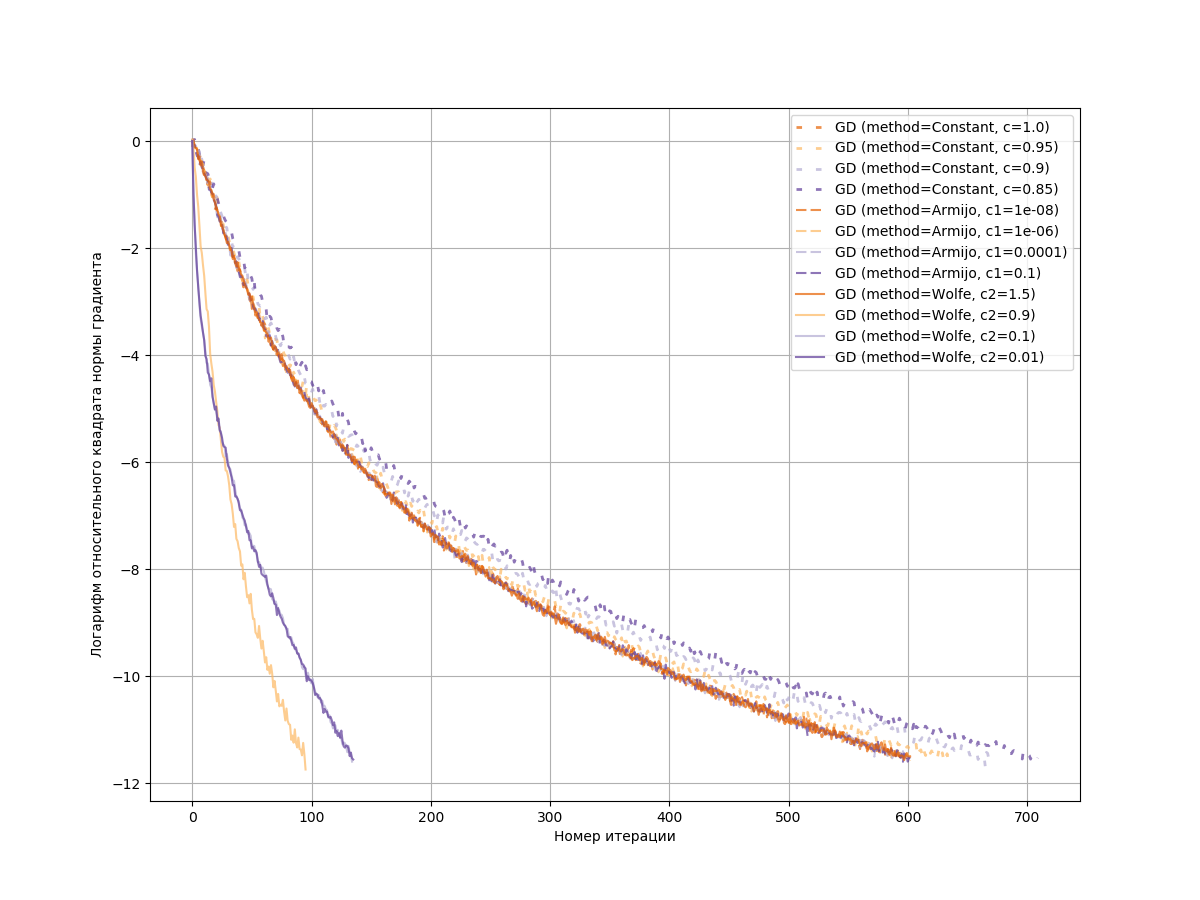
\includegraphics[width=.5\textwidth]{pics/logreg_GD_linear_search_strategies/x_0_1.png}
 		}
   \end{tabular}
	\subfloat[$x_0=1_n$]
		{
	    	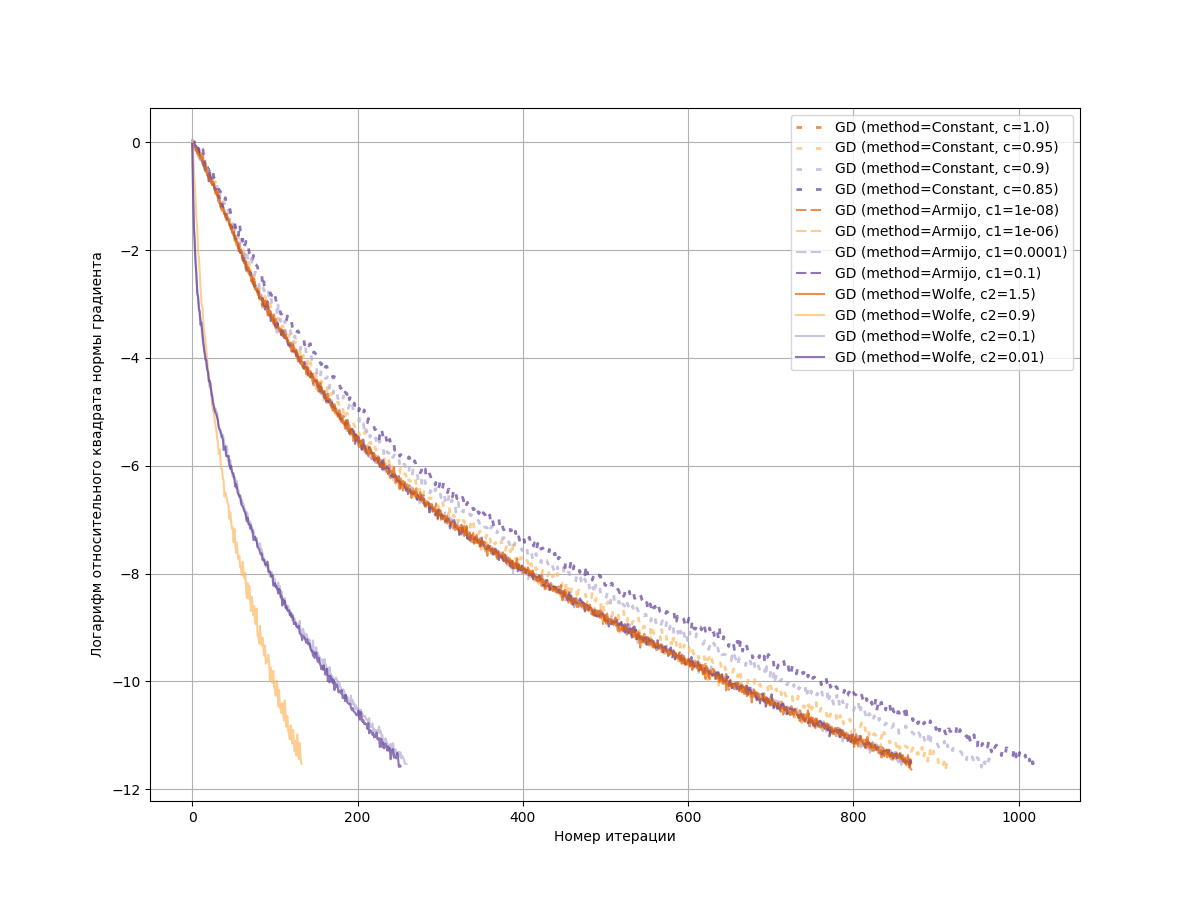
\includegraphics[width=.5\textwidth]{pics/logreg_GD_linear_search_strategies/x_0_2.png}
 		}
   \captionsetup{justification=centering}
   \caption{Графики зависимостей относительного квадрата градиента от номера итерации при использовании разных стратегий линейного поиска в GD (логистическая регрессия)}
\label{fig:gd_strategies_logreg}
\end{figure} 

\begin{figure}[h!p]
	\centering
	\begin{tabular}[c]{cc}
		\subfloat[$x_0=0_n$]{
    		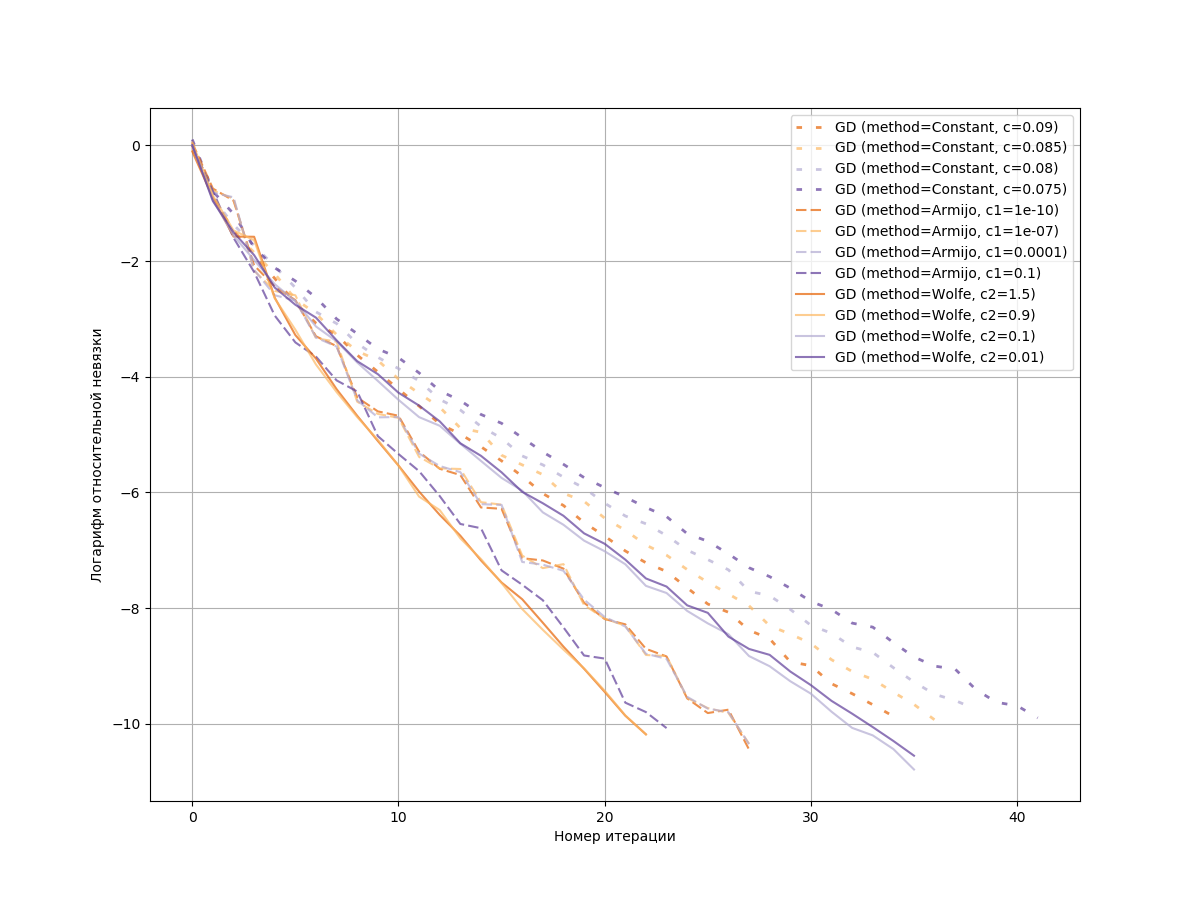
\includegraphics[width=.5\textwidth]{pics/quadratic_GD_linear_search_strategies/x_0_0.png}
 		} &

		\subfloat[$x_0$ -- случайная точка]{
    		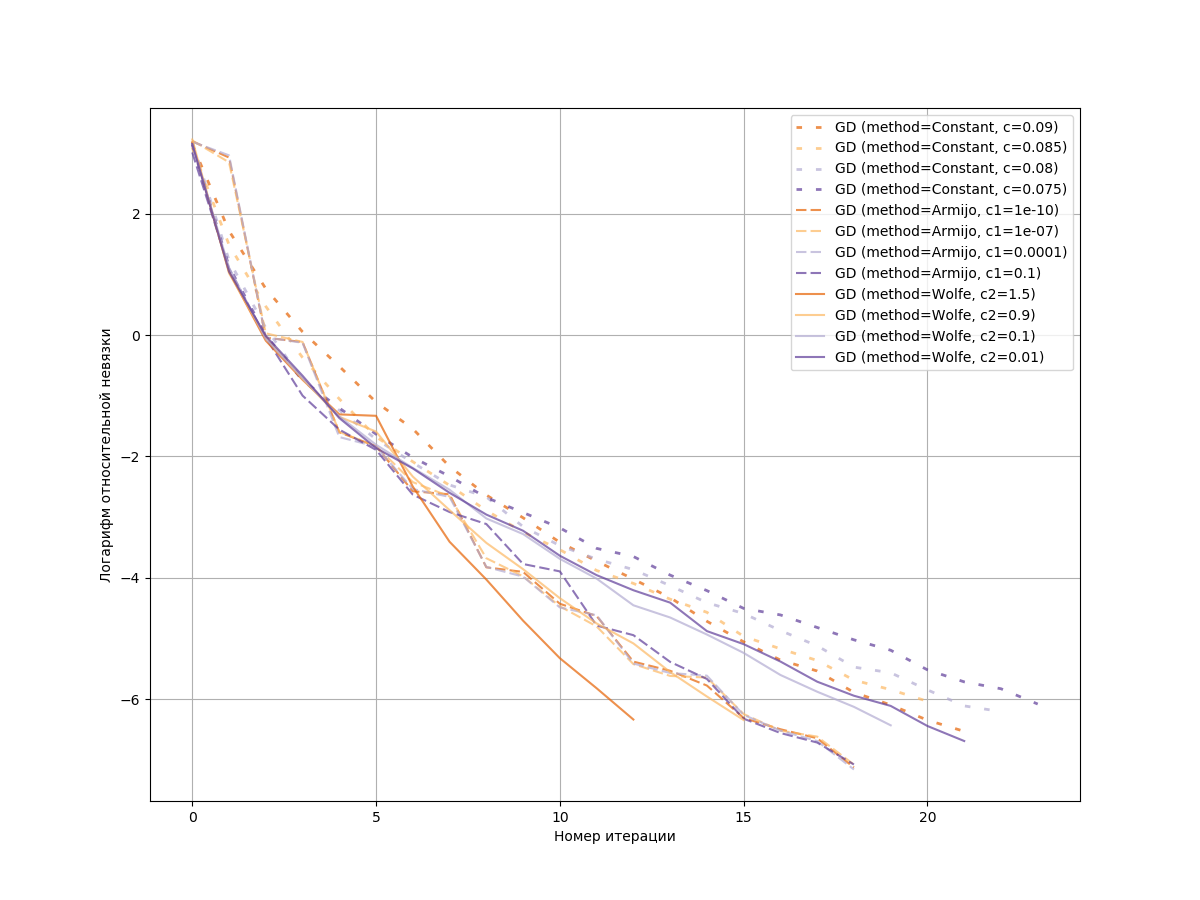
\includegraphics[width=.5\textwidth]{pics/quadratic_GD_linear_search_strategies/x_0_1.png}
 		}
   \end{tabular}
	\subfloat[$x_0$ -- оптимальная точка с добавлением шума]
		{
	    	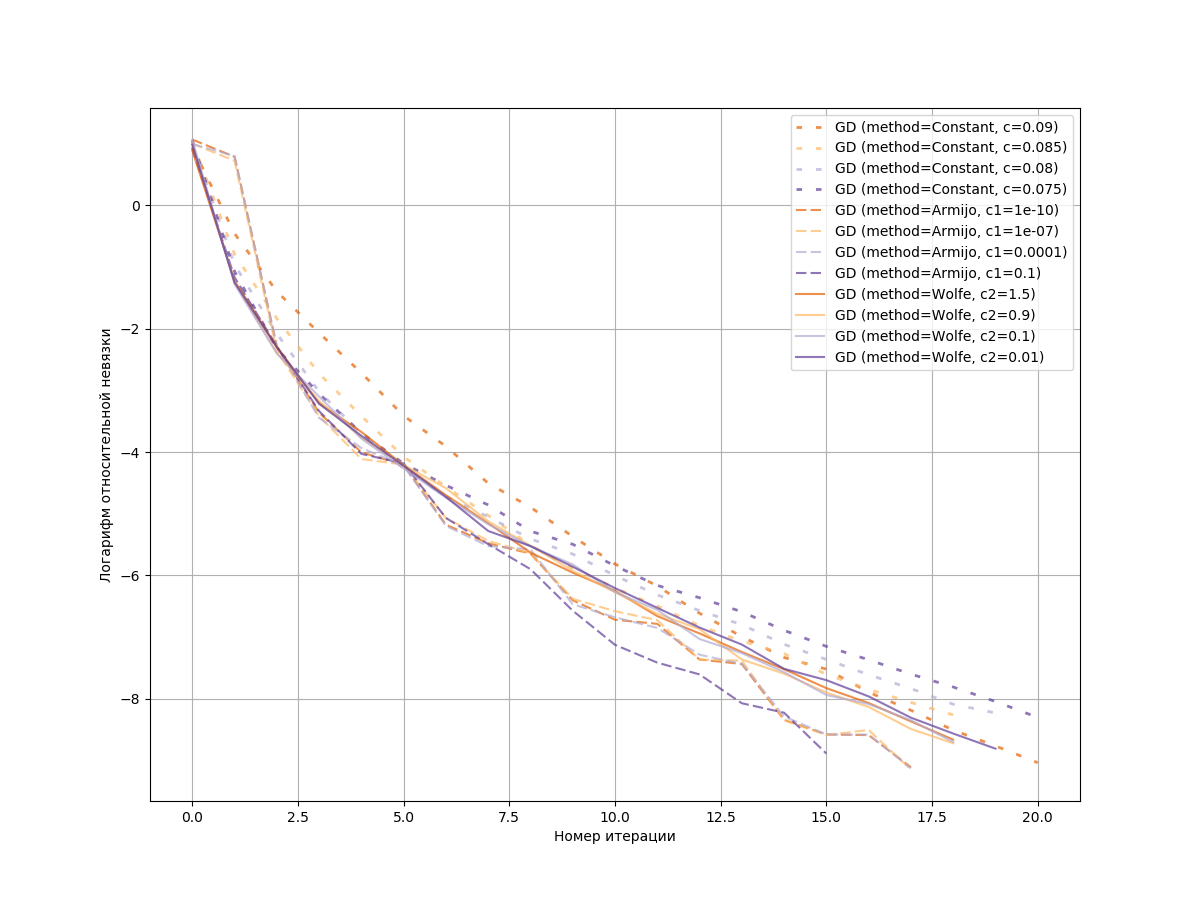
\includegraphics[width=.5\textwidth]{pics/quadratic_GD_linear_search_strategies/x_0_2.png}
 		}
   \captionsetup{justification=centering}
   \caption{Графики зависимостей относительной невязки от номера итерации при использовании разных стратегий линейного поиска в GD (оптимизация квадратичной функции)}
\label{fig:gd_strategies_quadratic}
	\end{figure}

\newpage
\subsection{Стратегия выбора длины шага в методе Ньютона}

Проведём аналогичный эксперимент с методом Ньютона. На рисунке \ref{fig:newton_strategies_logreg} можем увидеть, что лучшая стратегия -- использовать сильные условия Вульфа с $c_2 = 0.1$. Следом по возрастанию числа итераций идут другие стратегии с условиями Вульфа и стратегии с условием Армихо. Видно, что константная стратегия с теми же длинами шага, что использовались в предыдущем эксперименте, работает для метода Ньютона уже не со всеми начальными точками.

\begin{figure}[h!p]
	\centering
	\begin{tabular}[c]{cc}
		\subfloat[$x_0=0_n$]{
    		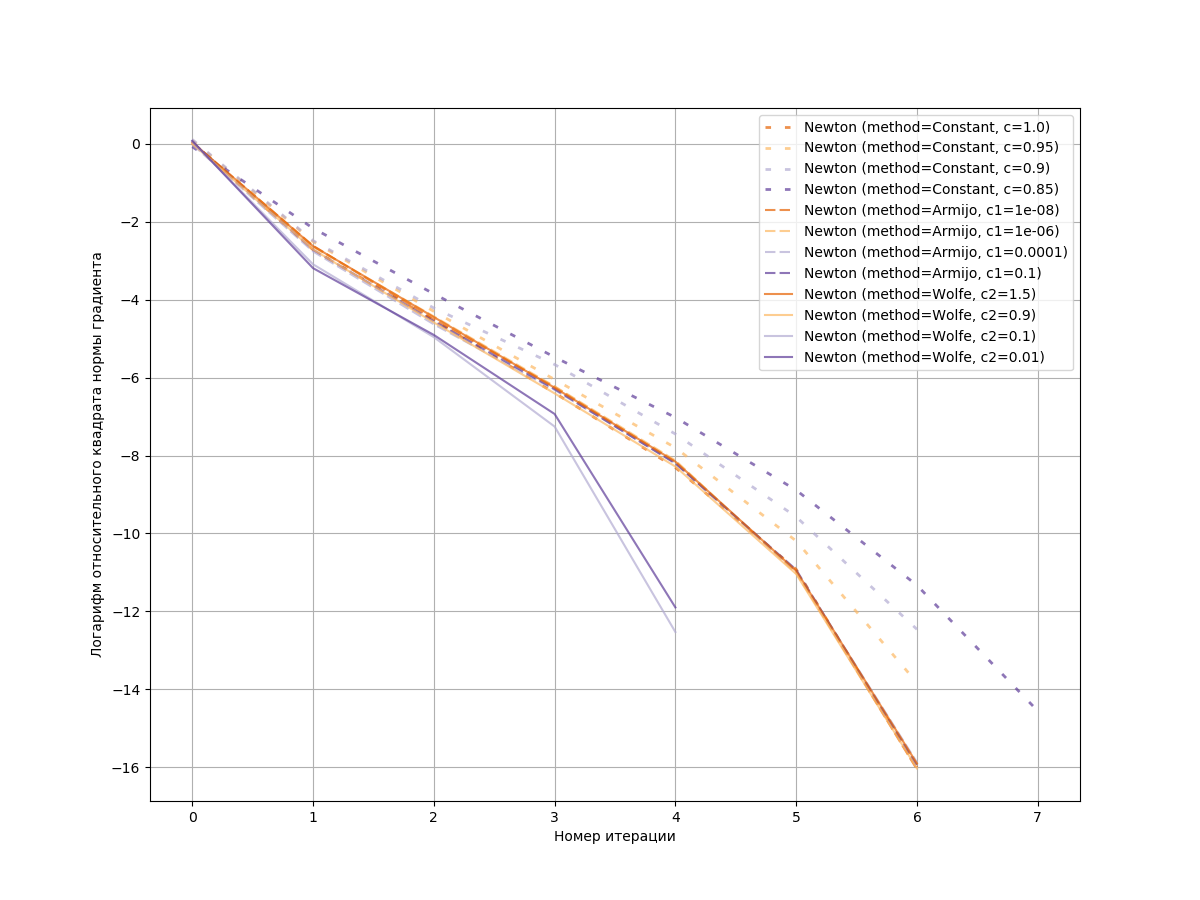
\includegraphics[width=.5\textwidth]{pics/logreg_Newton_linear_search_strategies/x_0_0.png}
 		} &

		\subfloat[$x_0$ -- случайная точка]{
    		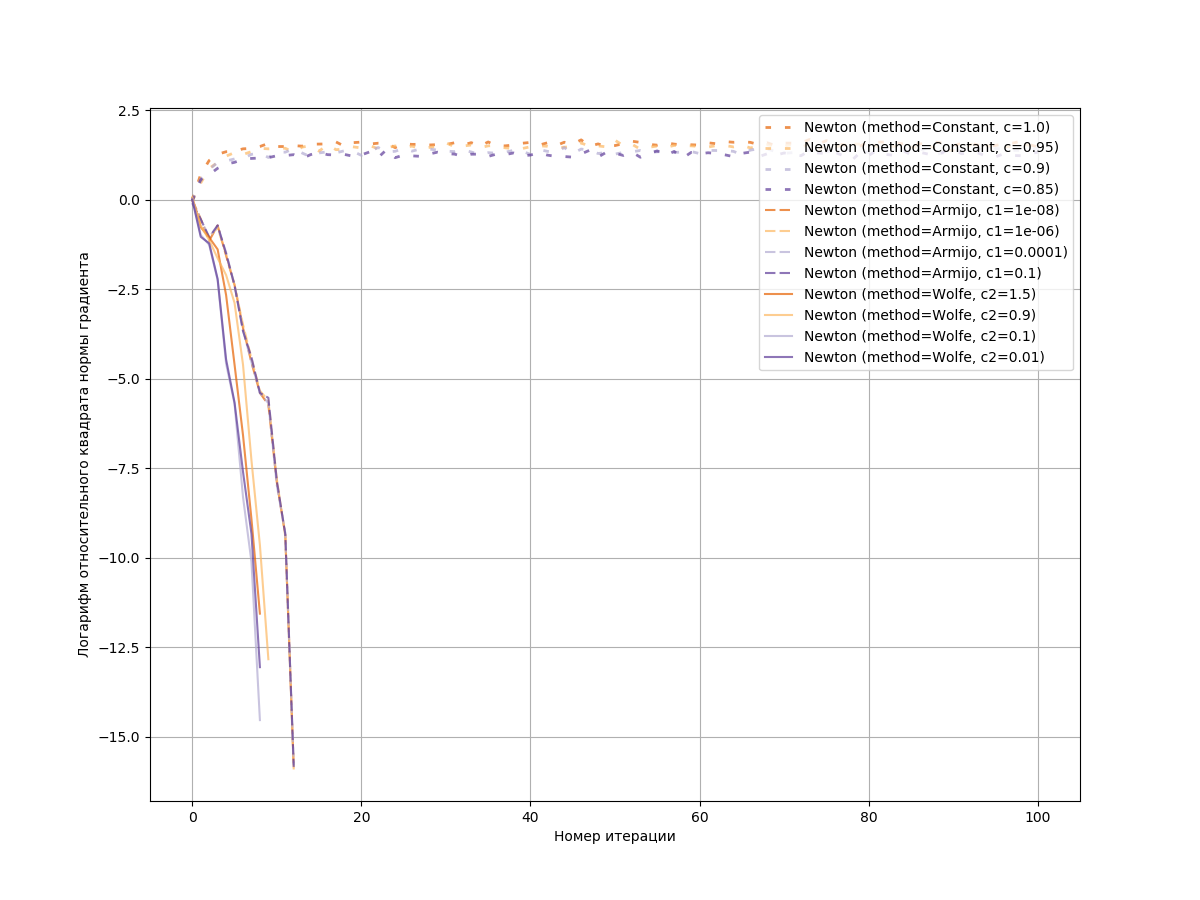
\includegraphics[width=.5\textwidth]{pics/logreg_Newton_linear_search_strategies/x_0_1.png}
 		}
   \end{tabular}
	\subfloat[$x_0=1_n$]
		{
	    	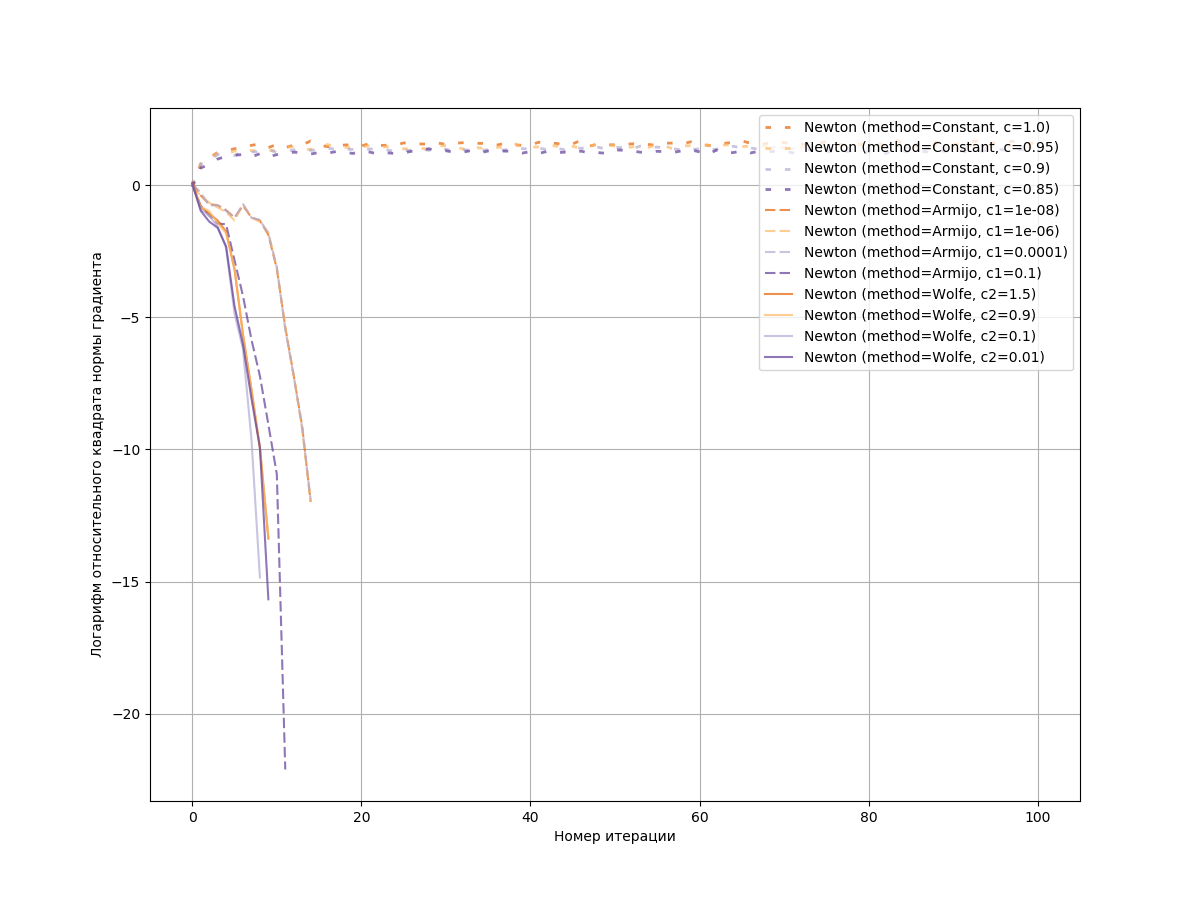
\includegraphics[width=.5\textwidth]{pics/logreg_Newton_linear_search_strategies/x_0_2.png}
 		}
   \captionsetup{justification=centering}
   \caption{Графики зависимостей относительного квадрата градиента от номера итерации при использовании разных стратегий линейного поиска в методе Ньютона (логистическая регрессия)}
\label{fig:newton_strategies_logreg}
\end{figure} 

\begin{figure}[h!p]
	\centering
	\begin{tabular}[c]{cc}
		\subfloat[$x_0=0_n$]{
    		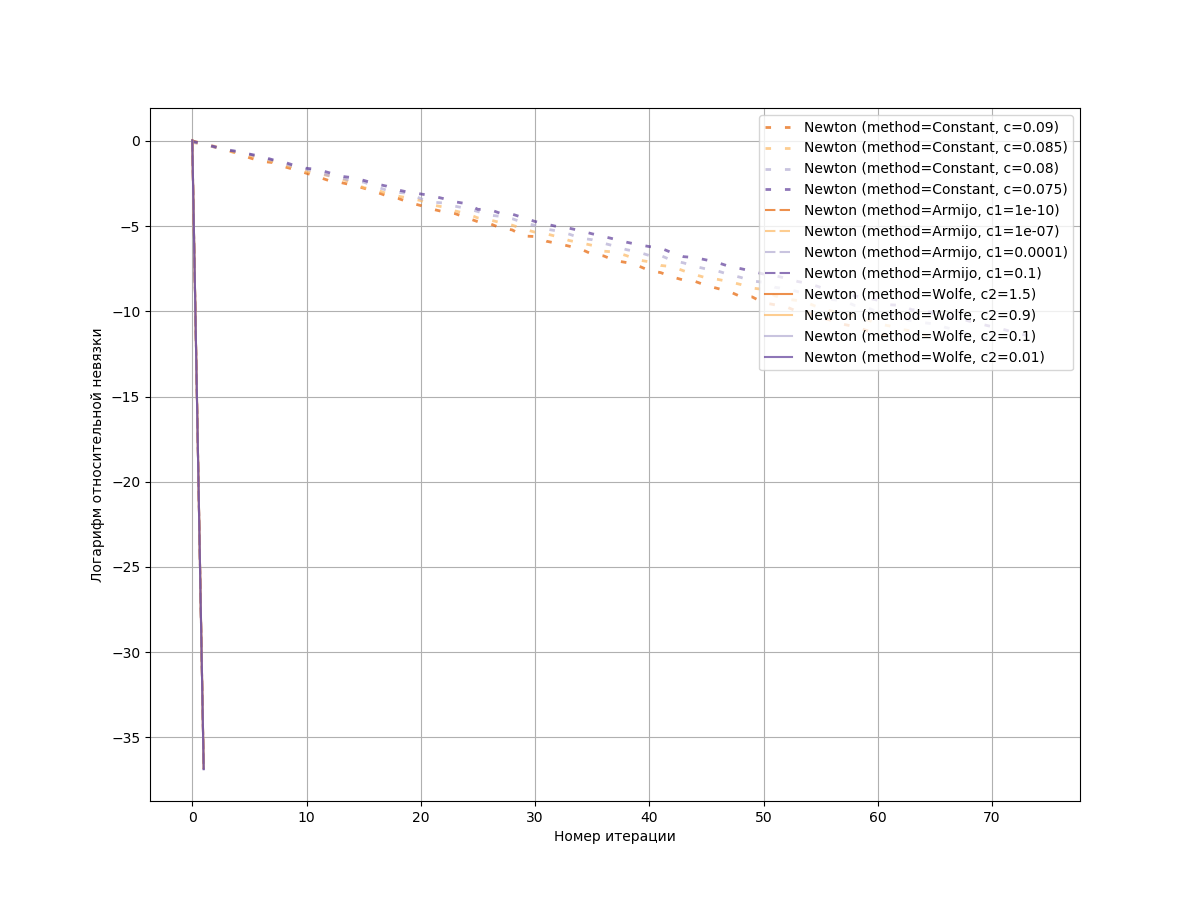
\includegraphics[width=.5\textwidth]{pics/quadratic_Newton_linear_search_strategies/x_0_0.png}
 		} &

		\subfloat[$x_0$ -- случайная точка]{
    		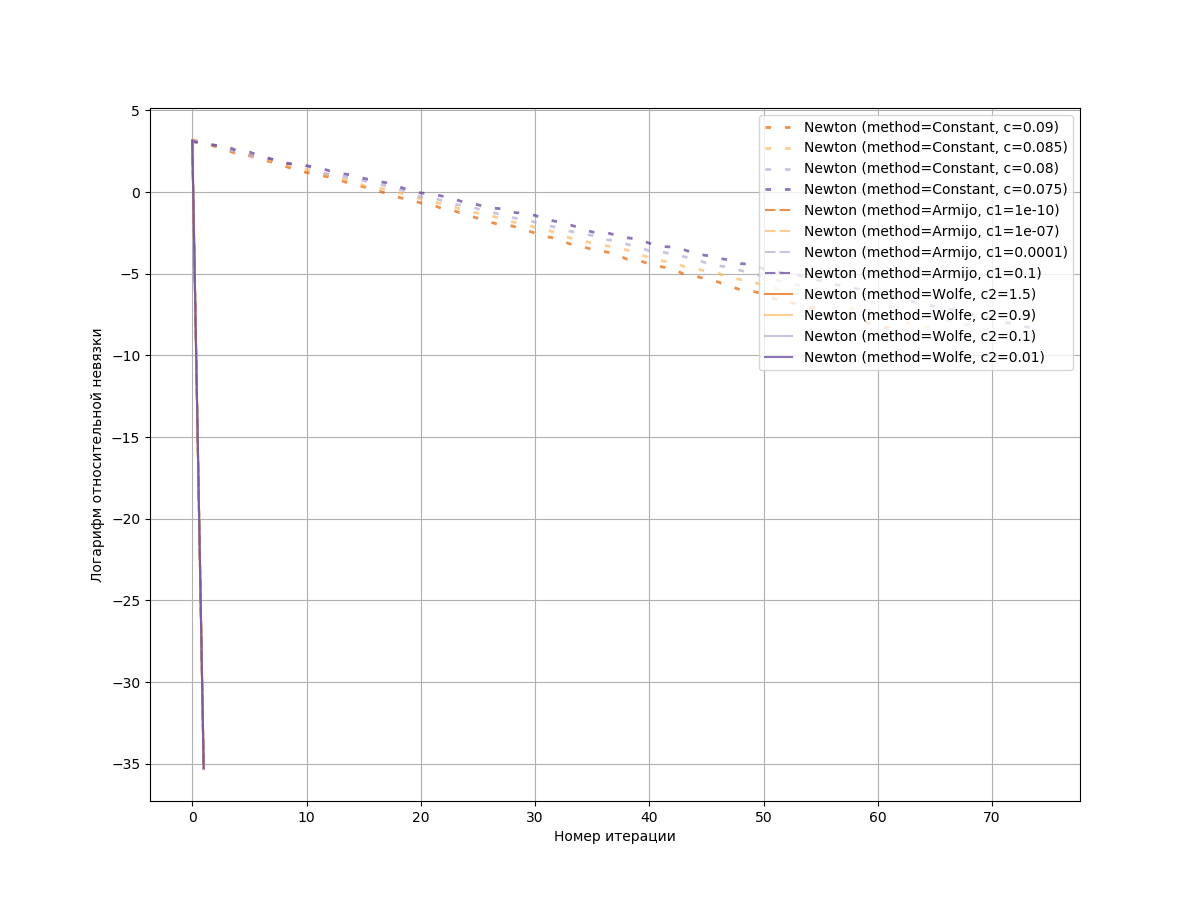
\includegraphics[width=.5\textwidth]{pics/quadratic_Newton_linear_search_strategies/x_0_1.png}
 		}
   \end{tabular}
	\subfloat[$x_0$ -- оптимальная точка с добавлением шума]
		{
	    	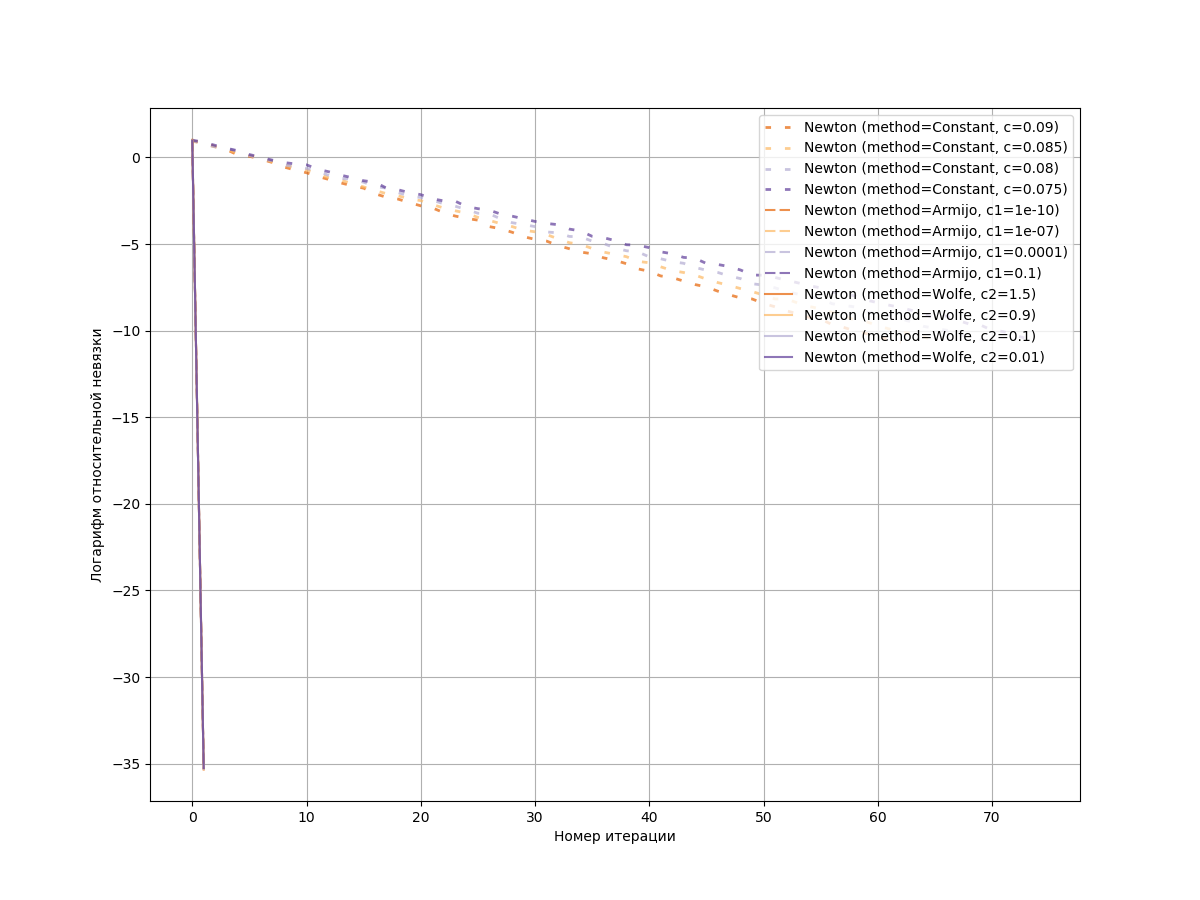
\includegraphics[width=.5\textwidth]{pics/quadratic_Newton_linear_search_strategies/x_0_2.png}
 		}
   \captionsetup{justification=centering}
   \caption{Графики зависимостей относительной невязки от номера итерации при использовании разных стратегий линейного поиска в методе Ньютона (оптимизация квадратичной функции)}
\label{fig:newton_strategies_quadratic}
\end{figure} 

На рисунке \ref{fig:newton_strategies_quadratic} все стратегии сходятся к оптимуму за одну итерацию, кроме константных (значение невязки в логарифмической шкале, вообще говоря, равно $-\infty$, но для возможности изобразить невязку на графике перед взятием логарифма было добавлено значение $\varepsilon=10^{-16}$), чего и следует ожидать -- метод Ньютона ищет оптимум квадратичной модели.

\section{Выводы.}
Мы изучили поведение градиентного спуска на разных функциях с использованием различных стратегий линейного поиска, увидели достоинства и недостатки метода Ньютона в сравнении с градиентным спуском (высокая скорость сходимости, но слишком высокая стоимость итерации, которая практически сводит на нет его преимущества). 

\end{document}